%====================================================================================
\section{Maximización del bienestar social: eficiencia y equidad}
%====================================================================================

\begin{frame}{Maximización del bienestar social en el espacio de utilidades:}
	\begin{figure}[!h]
		\centering
		\hspace{0.3cm}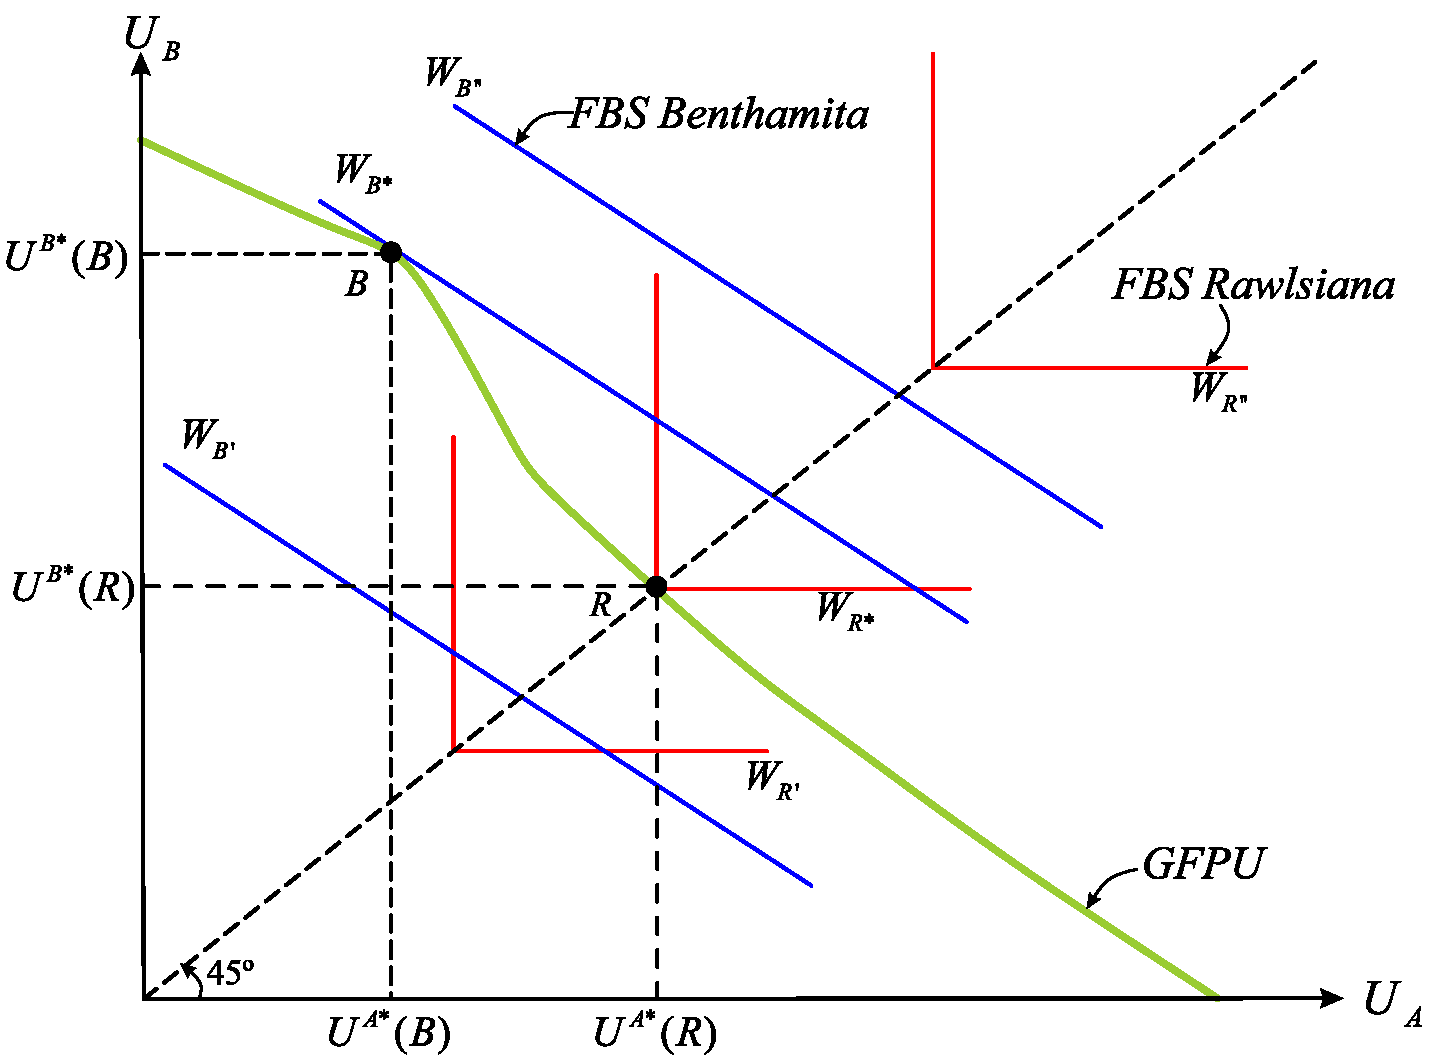
\includegraphics[width = 0.88\linewidth]{figures/fig_11.pdf}
	\end{figure}
\end{frame}
%------------------------------------------------
\begin{frame}{Optimo Social}
	La Gran Frontera de Utilidad debe ser tangente con el más alto contorno de indiferencia social (o FBS). Pendiente de la FBS:
			$$\frac{\partial W/\partial u^A}{\partial W/\partial u^B}$$
	Pendiente de la Gran Frontera de Utilidad: Si se transfiere una unidad de $X$ de $A$ a $B$, la ganancia de utilidad de $B$ respecto a la pérdida de utilidad de $A$ será:
		$$\frac{UMg_{X}^{B}}{UMg_{X}^{A}}$$	
	En general
		$$\frac{\partial W/\partial u^A}{\partial W/\partial u^B} = \frac{UMg_{X}^{B}}{UMg_{X}^{A}} = \frac{UMg_{Y}^{B}}{UMg_{Y}^{A}}$$
\end{frame}
%------------------------------------------------
\begin{frame}{Optimo Social}
	El punto óptimo social corresponde a la única mezcla de productos (X,Y) compatible con:
		\begin{itemize}
			\item Una asignación única de factores entre bienes $(K_X, K_Y, L_X, L_Y)$ que resuelve el problema de qué y cómo producir.
			\item Una asignación única de bienes entre personas $(X_A, X_B, Y_A, Y_B)$ que resuelve el problema de para quien producir.
		\end{itemize}
	Es decir, las condiciones para una organización económica ideal son:
		\begin{itemize}
			\item Eficiencia:
			\begin{itemize}
				\item Consumo eficiente $(TMS_A = TMS_B)$
				\item Producción eficiente $(TMST_X=TMST_Y)$
				\item Coordinación eficiente consumo - producción $(TMS=TMT)$
			\end{itemize}
			\item Justicia Social (Equidad)
		\end{itemize}
\end{frame}